\documentclass[12pt,a4paper]{scrartcl}
\usepackage[utf8]{inputenc}
\usepackage{siunitx}
\usepackage{graphicx}
\usepackage{amsmath}
\usepackage{float}
\usepackage{pdfpages}
\usepackage{circuitikz}

\newcommand{\n}[1]{\mkern 1.5mu\overline{\mkern-1.5mu#1\mkern-1.5mu}\mkern 1.5mu}
\newcommand{\g}[1]{\\\stackrel{\text{#1}}{=}}

\begin{document}
	\title{Grundlagen der Rechnerarchitektur\\ Übungsblatt 6}
	\date{}
	\author{Tarik Enderes, Jonas Strauch}
	\maketitle
	
	\begin{description}
		\item[1.] 
		\begin{description}
			\item[a)] 
			\begin{tabular}{c | c | c | c | c}
				$x_1$ & $x_2$ & $x_3$ & $x_4$ & $f(x)$\\\hline
				0 & 0 & 0 & 0 & 1 \\
				1 & 0 & 0 & 0 & 1 \\
				0 & 1 & 0 & 0 & 1 \\
				1 & 1 & 0 & 0 & 1 \\
				0 & 0 & 1 & 0 & 1 \\
				1 & 0 & 1 & 0 & 1 \\
				0 & 1 & 1 & 0 & 1 \\
				1 & 1 & 1 & 0 & 0 \\
				0 & 0 & 0 & 1 & 1 \\
				1 & 0 & 0 & 1 & 1 \\
				0 & 1 & 0 & 1 & 1 \\
				1 & 1 & 0 & 1 & 0 \\
				0 & 0 & 1 & 1 & 1 \\
				1 & 0 & 1 & 1 & 1 \\
				0 & 1 & 1 & 1 & 1 \\
				1 & 1 & 1 & 1 & 1 \\		
			\end{tabular}
			\item[b)] 
			\begin{math}
			f(x)=\n{x_1}\n{x_2}\n{x_3}\n{x_4}+x_1\n{x_2}\n{x_3}\n{x_4}+\n{x_1}\n{x_2}\n{x_3}\n{x_4}+x_1x_2\n{x_3}\n{x_4}+\n{x_1}\n{x_2}x_3\n{x_4}+x_1\n{x_2}x_3\n{x_4}+\n{x_1}x_2x_3\n{x_4}+\n{x_1}\n{x_2}\n{x_3}x_4+x_1\n{x_2}\n{x_3}x_4+\n{x_1}x_2\n{x_3}x_4+\n{x_1}\n{x_2}x_3x_4+x_1\n{x_2}x_3x_4+\n{x_1}x_2x_3x_4+x_1x_2x_3x_4
			\end{math}
			\item[c)] 
			\begin{math}
			f(x)=(\n{x_1}+\n{x_2}+\n{x_3}+x_4)\cdot(\n{x_1}+\n{x_2}+x_3+\n{x_4})
			\end{math}
			\item[e)] 
			\begin{tabular}{c | c | c | c | c | c}
				$ & \n{x_1} & x_1 & x_1 & \n{x_1} & \\\hline
				\n{x_2} & 1 & 1 & 1 & 1 & \n{x_4}\\\hline 
				x_2 & 1 & 1 & 0 & 1 & \n{x_4}\\\hline
				x_2 & 1 & 0 & 1 & 1 & x_4\\\hline
				\n{x_2} & 1 & 1 & 1 & 1 & x_4\\\hline   
				& \n{x_3} & \n{x_3} & x_3 & x_3 & \\$
			\end{tabular}\\
		\begin{math}
			\implies f(x) = \n{x_1}+\n{x_2}+\n{x_3}\n{x_4}+x_3x_4
			
		\end{math}
		\item[e)] 
		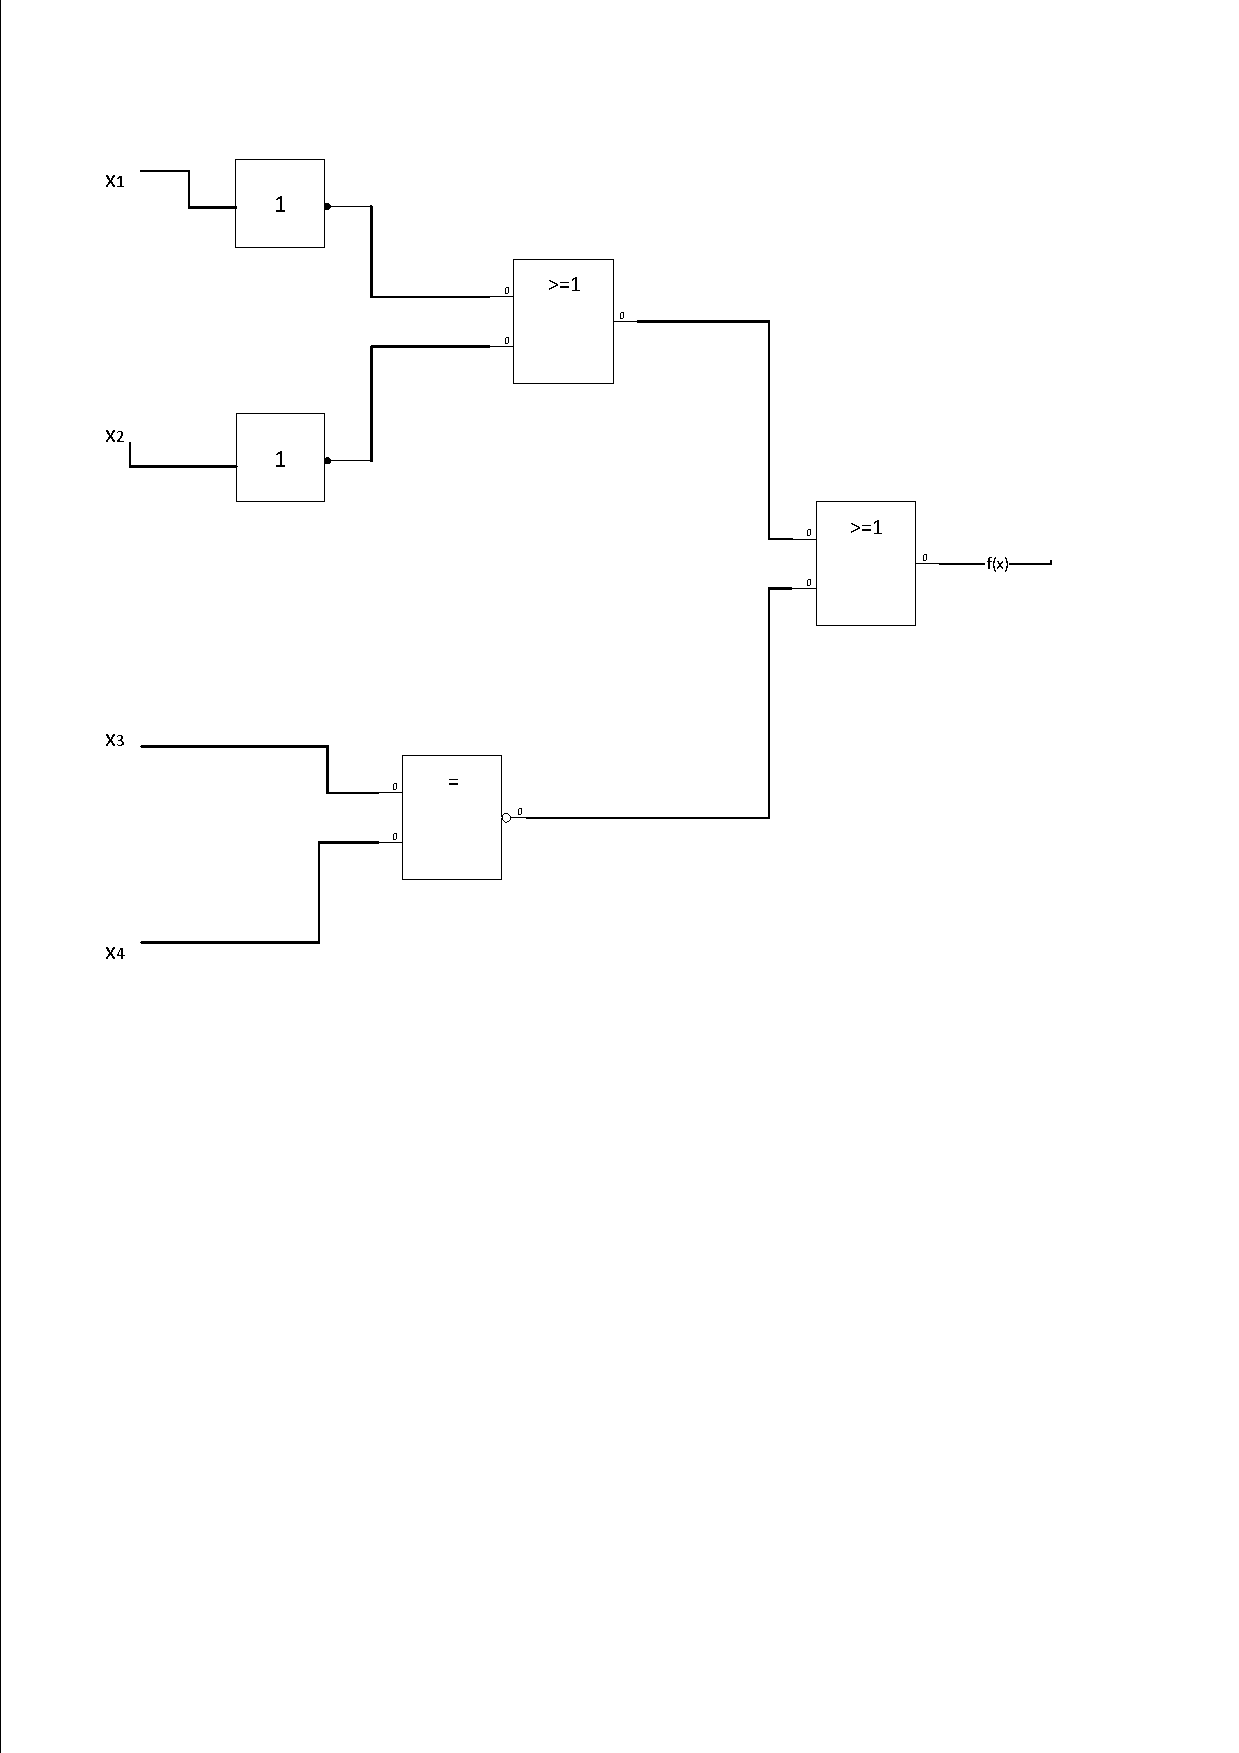
\includepdf[pages=-]{Blatt6_1_f.pdf}
		\end{description}
	\item[2.]
	\begin{description}
		\item[a)] Bei Gattern, die mit N-mos oder P-mos aufgebaut sind, wird eine 0 am Ausgang realisiert, indem der Strom durch die Erdung abgeleitet wird. Diese Gatter haben in diesem Fall deshalb eine hohe Leistungsaufnahme und erwärmen sich entsprechend. Bei C-mos-Gattern fließt nur beim Umschalten zwischen den Zuständen Strom. Der Energieverbrauch ist also niedriger.
		\item[b)]
		\begin{math}
		f(x_1, x_2, x_3) = \n{x_1x_2+x_2x_3}
		\end{math}
		\item[c)] 
		\begin{tabular}{c | c | c | c}
			$x_1$ & $x_2$ & $x_3$ & $f(x)$\\\hline
			0 & 0 & 0 & 1 \\
			1 & 0 & 0 & 1 \\
			0 & 1 & 0 & 1 \\
			1 & 1 & 0 & 0 \\
			0 & 0 & 1 & 1 \\
			1 & 0 & 1 & 1 \\
			0 & 1 & 1 & 0 \\
			1 & 1 & 1 & 0 \\	
		\end{tabular}
	\end{description}
	\end{description}
\end{document}